\chapter{Evaluation}

\section{\bb 3}
\begin{wrapfigure}{r}{0.4\textwidth}
	\centering
	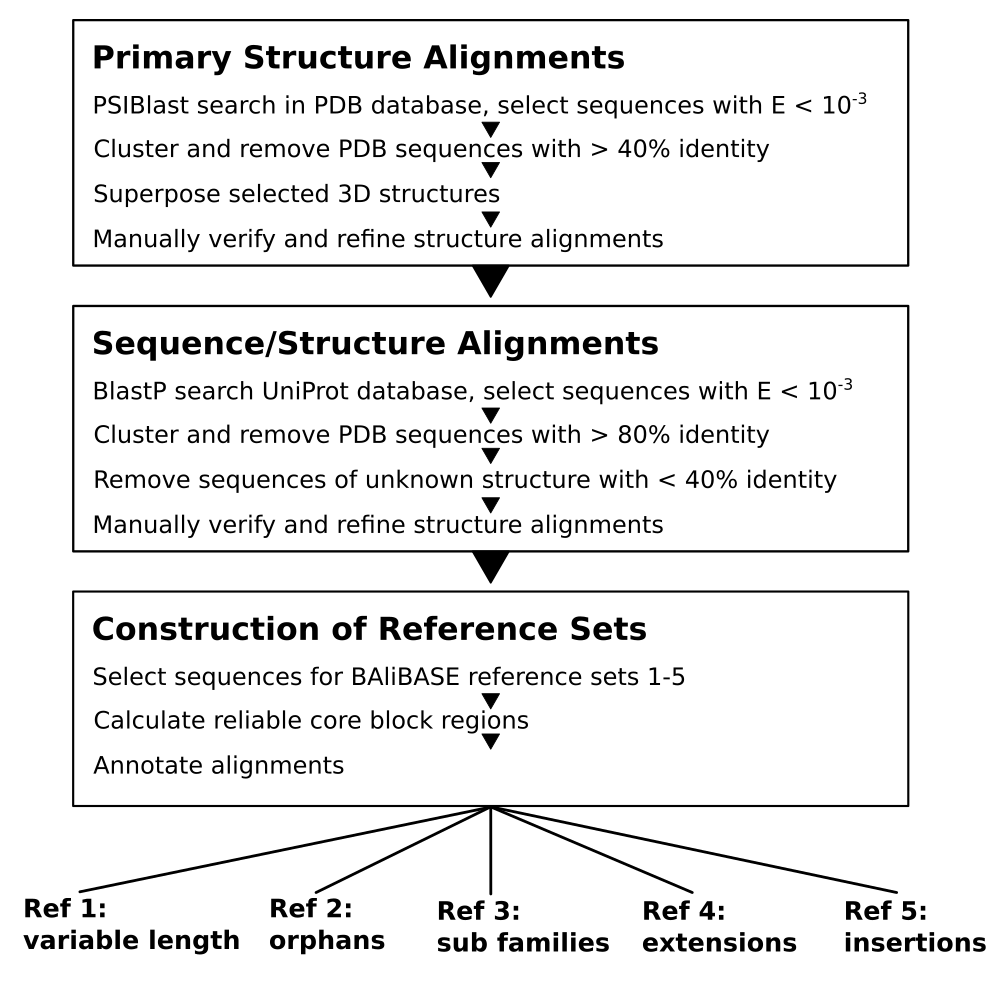
\includegraphics[width=0.5\textwidth]{./images/balibase.png}
	\caption{Flow chart showing the semi automatic process used to establish the reference sets TODO cite self}
	\label{fig:balibase}
\end{wrapfigure}

The third version of the \bb benchmark protein alignment database has been released in 2005 and is widely employed for the comparison of multiple alignment programs \cite{thompson2005balibase, Russell2016}. It is constructed in a semi automatic process as shown in \cref{fig:balibase} and suitable to evaluate global and local alignment programs. The database is split into 5 reference sets with different characteristics representing distinctive multiple alignment problems.



\begin{itemize}
	\item reference set 1 subset V1, for which any two sequences share <20\% identity and no internal insertions over 35 residues long
	\item reference set 1 subset V2, consisting of families with at least four equidistant sequences for which any two sequences share 20-40\% identity and no large insertions
	\item reference set 2, for which all sequences share >40\% identity and at least one 3D structure is known. Additionally an "Orphan" sequence with <20\% identity is chosen per family
	\item for reference set 3, all sequences in the same subfamily have >40\% identity, whereas sequences from different subfamilies share <20\% identity
	\item for reference sets 4 and 5, every sequence shares at least 20\% with one other sequence, including sequences with large N/C-terminal extensions (ref 4) or internal insertions (ref 5)
\end{itemize}

\subsection{Core blocks}




\section{Sum-of-pairs and column score}

\section{MAFFT}

\section{Results}
